\documentclass[12pt,a4paper]{report}
\renewcommand{\bibname}{References}
\usepackage{url}
\usepackage{hyperref}
\usepackage{pdfpages}
\usepackage{titlesec, blindtext, color}
\usepackage{amsmath}
\usepackage{amsfonts}
\usepackage{algorithm}
\usepackage{needspace}
\usepackage{algorithmic}
\usepackage{graphicx}
\usepackage{geometry}
\usepackage{relsize} 
\usepackage{placeins}
\usepackage{wrapfig}
\usepackage{setspace}
\usepackage{natbib}
\citestyle{nature}
\usepackage{amsthm}
\usepackage{subfiles}
\usepackage[utf8]{inputenc}
\usepackage{multirow}
\usepackage{booktabs}
\usepackage[bottom]{footmisc}
\usepackage[nottoc]{tocbibind} 
\usepackage[font=footnotesize, labelfont=bf]{caption}
\captionsetup[table]{position=below}
\captionsetup[figure]{position=below}

\graphicspath{ {images/} }

\titleformat{\chapter}[block]
  {\normalfont\huge\bfseries}{\thechapter.}{1em}{\Huge}
\titlespacing*{\chapter}{0pt}{35pt}{50pt}

\newcommand{\hsp}{\hspace{20pt}}
\newcommand{\code}{\texttt}

\begin{document}

\newgeometry{margin=1in}
\begin{titlepage}
        
        \noindent
        \begin{minipage}[t]{0.19\textwidth}
            \vspace{-4mm}{
\includegraphics[scale=1.15,draft=false]{images/logo_unimib.pdf}}	
        \end{minipage}
    \hspace{2mm}
    \begin{minipage}[t]{0.81\textwidth}
    {	\setstretch{2.1}
            {\textsc{Università degli Studi di Milano - Bicocca}} \\
            \textbf{Dipartimento di Informatica, Sistemistica e Comunicazione} \\
            \textbf{Corso di Laurea in Informatica} \\
            \par
    }
    \end{minipage}
    
\vspace{40mm}
    
\begin{center}
        {\Huge{
                \textbf{Detection of Genomic Inversions Using Sample-Specific Strings}
                \par
        }}
    \end{center}
    
    \vspace{50mm}

    \noindent
    {\large \textbf{Relatore:} Prof.ssa Paola Bonizzoni} \\

    \noindent
    {\large \textbf{Correlatore:} Dott. Luca Denti}
    
    \vspace{15mm}

    \begin{flushright}
        {\large \textbf{Tesi di Laurea di:}} \\
        \large{Silvia Cambiago} \\
        \large{Matricola 879382} 
    \end{flushright}
    
    \vspace{20mm}
    \begin{center}
        {\large{\bf Anno Accademico 2023-2024}}
    \end{center}
   
\end{titlepage}
\restoregeometry



\thispagestyle{empty}

\begin{flushright}
\textit{
You gotta dig deep, and bury all the thoughts \\
The thoughts that tell you, you're not good enough\\
The critics, the cynics, say you'll never make it\\
Prove 'em all wrong, they are mistaken\\
}

\medskip
\textit{Hold on, 'cause you don't know what is going to happen\\
Stay strong, your life's worth more than you know}

\bigskip

\textit{
\textbf{I Prevail - Crossroads}}

\end{flushright}

\begin{abstract}
This thesis presents the development of an efficient algorithm that detecting genomic inversions using sequencing data, specifically focusing on long reads and using sample-specific strings to identify the inversions. \\
It begins by introducing the concept of inversions, explaining their biological meaning, and providing a detailed overview of the data structures and definitions that form the basis of the algorithm. \\
The algorithm itself is then thoroughly described, with a complete theoretical analysis of its design, its computational complexity and the logic that lies behind it. \\
Later on, the thesis covers the practical implementation and experimentation, that was performed using the SVDSS tool to validate the algorithm. The results are finally summarized and discussed, demonstrating the algorithm's effectiveness.

\end{abstract}
\addtocounter{page}{0} 

\tableofcontents

\chapter{Introduction}
\section{Context} 

Inversions, as defined by HGVS \cite{noauthor_inversion_nodate} (Human Genome Variation Society), are sequence changes where, compared to a reference sequence, more than one nucleotide replacing the original sequence is the reverse complement of the original sequence. They are a category of genomic structural variations (SVs), defined as alterations in the DNA that affect more than 50 bp that may delete, insert, duplicate, invert, or move genomic sequences \cite{eslami_rasekh_discovery_2017} (see Figure \ref{fig:svs}). 

\begin{figure}[h]

  \centering
    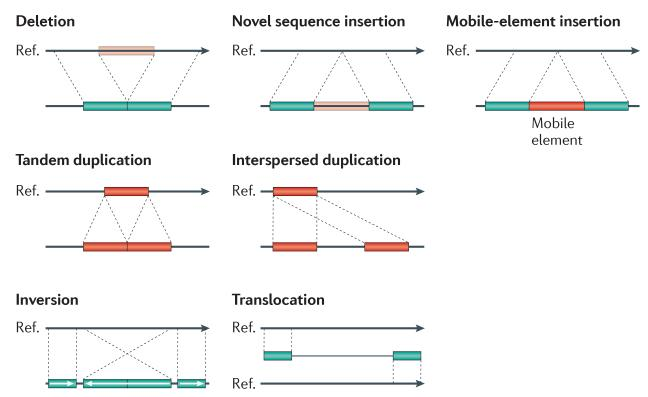
\includegraphics[width=250px]{svs.jpg}

  \caption{Outline of different SV-archetypes.}
  \label{fig:svs}
\end{figure}

They are often generated by non-allelic homologous recombination (NAHR) between inverted repeats, but they can also be originated by double-strand break repair mechanisms, like non-homologous end joining (NHEJ), or replication-based mechanisms mediated by microhomology, like fork stalling and template switching \cite{puig_human_2015}. Although inversions constitute only a small fraction of SVs across various organisms, ranging from 0.5\% to 7\% \cite{hu_unravelling_2024}, they can span over 100 Mb and collectively account for up to 10\% of the genome, holding considerable functional and evolutionary significance. \\


Inversions were first identified in 1917 by Alfred Sturtevant \cite{sturtevant_case_1921}, and he found out they act as suppressors of recombination between chromosomes. Since then, inversions have been drawing increasing attention, due to their crucial role in driving genome evolution and their link to the evolutionary processes of many species. In fact, it was later found that suppressed recombination among genes within an inversion can lead to largely independent genome evolution between derived and ancestral arrangements, providing opportunities for divergence and speciation \cite{faria_evolving_2019}. This genomic isolation, facilitated by inversions, can lead to the formation of novel genotypes and phenotypes, contributing to the genetic diversity we can observe today. \\

But inversions are not only related to evolution. In fact, they are involved in the formation of several diseases, as will be shown in Chapter 2. A recent study even shows that the contribution of chromosomal inversions to phenotypic diversity can even affect brain development and lead to disorders \cite{wang_chromosomal_2023}.

\section{Inversions detection}

Due to their significance, the challenge of detecting inversions has been widely addressed. The first methods developed for this scope, such as cytogenetics or PCR-based approaches, were labor‐intensive and lacked resolution, limiting their effectiveness \cite{hu_unravelling_2024}. With the advent of high-throughput next-generation sequencing (NGS), large-scale population studies of inversions became finally possible, enabling the discovery of polymorphic inversions and their association with phenotypic traits.
In addition to this, long‐read DNA sequencing technologies such as PacBio HiFi sequencing or Oxford Nanopore duplex sequencing have enabled the generation of sequencing reads between 10  kb and 2  Mb, making them highly useful for detecting inversions. Therefore, identifying inversions has become more straightforward with the use of long reads that can span repetitive and complex genomic regions. However, despite all this technological progress, inversions remain one of the most underascertained forms of structural variation in human and non-human primate genomes, limiting our understanding of their evolution significance \cite{porubsky_recurrent_2020}. The main challenge continues to be the precise determination of inversion breakpoints.

\section{Project}

In this thesis will be presented an algorithm designed to detect the presence of genomic inversions from long-read sequencing data using sample-specific strings (which will be defined in detail in Chapter 2) to determine the breakpoints. A \texttt{Python} implementation of the algorithm will be used for the practical experimentation, in combination with the SVDSS \cite{denti_svdss_2023} tool, that will also be implemented in the code and will help in detecting the number, position, and length of the sample-specific strings. \\
\\
In Chapter 2, the necessary preliminaries will be presented to understand how the algorithm works, including the definitions used throughout the thesis and the biological background that lies behind inversions, other than their pratical biological consequences. \\
In Chapter 3, the algorithm will be presented in detail, including the pseudocode and a complete theoretical analysis. This chapter will treat, among other things, time and space complexity and proof of correctness.\\
In Chapter 4, the practical experimentation will be discussed, explaining the \texttt{Python} implementation of the code and the use of the SVDSS tool. The results will be presented, summarized, and commented upon.

\bigskip
\bigskip



\chapter{Preliminaries}
\newtheorem{definition}{Definition}
\newtheorem{example}{Example}

The algorithm's primary objective is to detect reverted sequences within a target DNA sequence, which are characterized by segments that have been inverted and complemented relative to a reference DNA sequence. \\
It uses sample-specific strings as possible anchors of an inverted portion occurring in the target.

\section{Definitions}
In this paragraph will be introduced the definitions that will be used throughout the thesis. \\
The definition of sample-specific string\cite{khorsand_comparative_2021} is as follows:

\begin{definition}[Sample-specific string (SFS)]
A sample-specific string S is a string that occurs in the target DNA string T, does not occur in the reference DNA string R, and for every string S' which is a substring of S, S' occurs in the reference string R. 
\label{thm:sample_specific}
\end{definition} 

Subsequently, it will be necessary to formally define what constitutes an inverted segment of the target $T$ in relation to the reference $R$. The following definitions establish these key concepts:

\begin{definition}[Inversion]
Let $T$ be a target string and $R$ a reference string. A substring $s = T[i,j]$ for $1 \leq i < j \leq |T|$ is a single inversion in the target $T$ with respect to $R$ if $s^{rc}$ occurs as a substring of $R$. If the inversion in $T$ occurs from $i$ to $j$, it is denoted as a triple $(T, i, j)$.
\end{definition}

Next, the concept of substring from $i$ to $j$ is defined, along with the notion of a single inversion:

\begin{definition}[Substring]
Given a string \( S \), the substring \( S[i:j] \) is defined as the sequence of characters in \( S \) that starts at position \( i \) (inclusive) and ends at position \( j \) (exclusive). Formally, \( S[i:j] = s_i s_{i+1} \ldots s_{j-1} \), where \( s_k \) represents the character at position \( k \) in the string \( S \), and \( 0 \leq i < j \leq |S| \).
\end{definition}

\begin{definition}[Single Inversion]
Given a string $S$, another string $S'$ is obtained by a single inversion on $S$ from $i$ to $j$ if $S'$ is derived by reversing and complementing $S[i,j]$, denoted as $S[i,j]^{rc}$.
\end{definition}

Finally, the concept of inversion breakpoint is introduced:

\begin{definition}[Inversion Breakpoint]
Given an inversion $(S', i, j)$ in string $S'$ with respect to string $S$, the indexes $i$ and $j$ are referred to as breakpoints of the inversion if $S[i,j] = S'[i,j]^{rc}$, and no index $i' < i$ or $j' > j$ exists such that $S[i',j'] = S'[i',j']^{rc}$.
\end{definition}

These definitions will be used in the description of the algorithm for solving the Detecting-Inversions problem, described in Chapter 3. In cases involving multiple inversions, the target may result from several disjoint inversions.\\

Since the Knuth-Morris-Pratt algorithm will be introduced in Section 2.4 below as the method used to verify the presence of the middle segment between two sample-specific strings (extracted from the target) within the reference, a few clarifying definitions\footnote{https://proofwiki.org/wiki/Definition:Prefix} are presented here:

\begin{definition}[Proper prefix]
Given a string $S$, a string $T$ is a prefix of $S$ if and only if $S$ can be formed by concatenating $T$ with another string $T'$. If $S = TT'$, $T$ is a proper prefix of $S$ if $T' \neq \varepsilon$, meaning $T'$ is not the empty string.

\label{thm:proprefix}
\end{definition}

\begin{definition}[Proper suffix]
Given a string S, a string T is a suffix of S if and only if S can be formed by concatenating another string T' with T. If $S = TT'$, $T'$ is a proper suffix of $S$ if $T \neq \varepsilon$, meaning $T$ is not the empty string.
\label{thm:prosuffix}
\end{definition}

\section{Biological Background}

\subsection{DNA}

Before addressing the computational part of the project, it is useful to present an overview of its biological background. \\
Deoxyribonucleic acid (DNA) is the molecule that carries genetic information for the development and functioning of an organism\footnote{https://www.genome.gov/genetics-glossary/Deoxyribonucleic-Acid}. Each DNA molecule consists of a long polymer made up of repeating units, the nucleotides, which are composed of a phosphate group, a sugar molecule, specifically 2-deoxyribose, and a nitrogenous base. There are four types of nitrogenous bases found in DNA that define the properties of the nucleotide: adenine (A), thymine (T), guanine (G), and cytosine (C), as shown in Figure \ref{fig:dna}.\\

\begin{figure}[h]

  \centering
    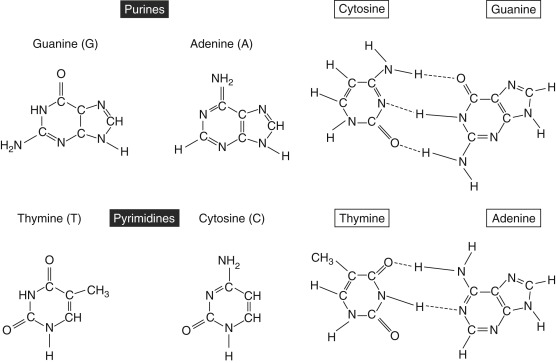
\includegraphics[width=250px]{dna.jpg}

  \caption{DNA nucleotide bases and base pairing.}
  \label{fig:dna}
\end{figure}

In all eukaryotic organisms, DNA exists as a tightly associated pair of two long strands that intertwine, forming the shape of a double helix. The two strands of DNA are stabilized by hydrogen bonds between the nitrogenous bases attached to the two strands \cite{carter_chapter_2022}. Watson-Crick base pairing involves adenines pairing with thymines and guanines pairing with cytosines. Strands of DNA that form matches among base pairs are called complementary strands. \\

\subsection{Double strand breaks}

Double-strand break (DSB) is the primary cytotoxic lesion generated by ionizing radiation, radio-mimetic chemicals such as camptothecin (CPT), mechanical stress on chromosomes, or when the replication machinery encounters a single-strand DNA break or other types of DNA lesions. In addition to this, DSBs can also be produced during physiological processes, such as recombination or meiosis \cite{ting_rad18_2010}.
DSBs are a particularly dangerous form of DNA damage because they can lead to chromosome loss, translocations or truncations. Repair occurs via one of two pathways: non-homologous end-joining (NHEJ), in which broken DNA ends are directly ligated; or homologous recombination (HR), in which a homologous chromosome is used as a template in a replicative repair process. 

\subsection{DNA recombination and formation of inversions}

Genetic recombination is a fundamental cellular process that has a role in the generation of genetic diversity, in the repair of damaged DNA, in the homologous alignment of chromosomes required for successful completion of meiotic cell division, and in the generation of genomic alterations that lead to changes in gene expression. Classical homologous recombination is a type of genetic recombination in which nucleotide sequences are exchanged between two similar or identical molecules of DNA, as shown in Figure \ref{fig:hr}. During the formation of egg and sperm cells (meiosis), paired chromosomes from the male and female parents align so that similar DNA sequences can cross over, or be exchanged, from one chromosome to the other. This exchange of DNA is an important source of the genomic variation seen among offspring\footnote{https://www.genome.gov/genetics-glossary/homologous-recombination}.
This allelic homologous recombination repairs double-stranded breaks (DSBs) in chromosomes by using the allele on the sister chromatid as a template. This mechanism is highly faithful because the allelic region of the sister chromatid is a nearly exact copy of the DNA lost in the DSB \cite{parks_detecting_2015}. 

\begin{figure}[h]

  \centering
    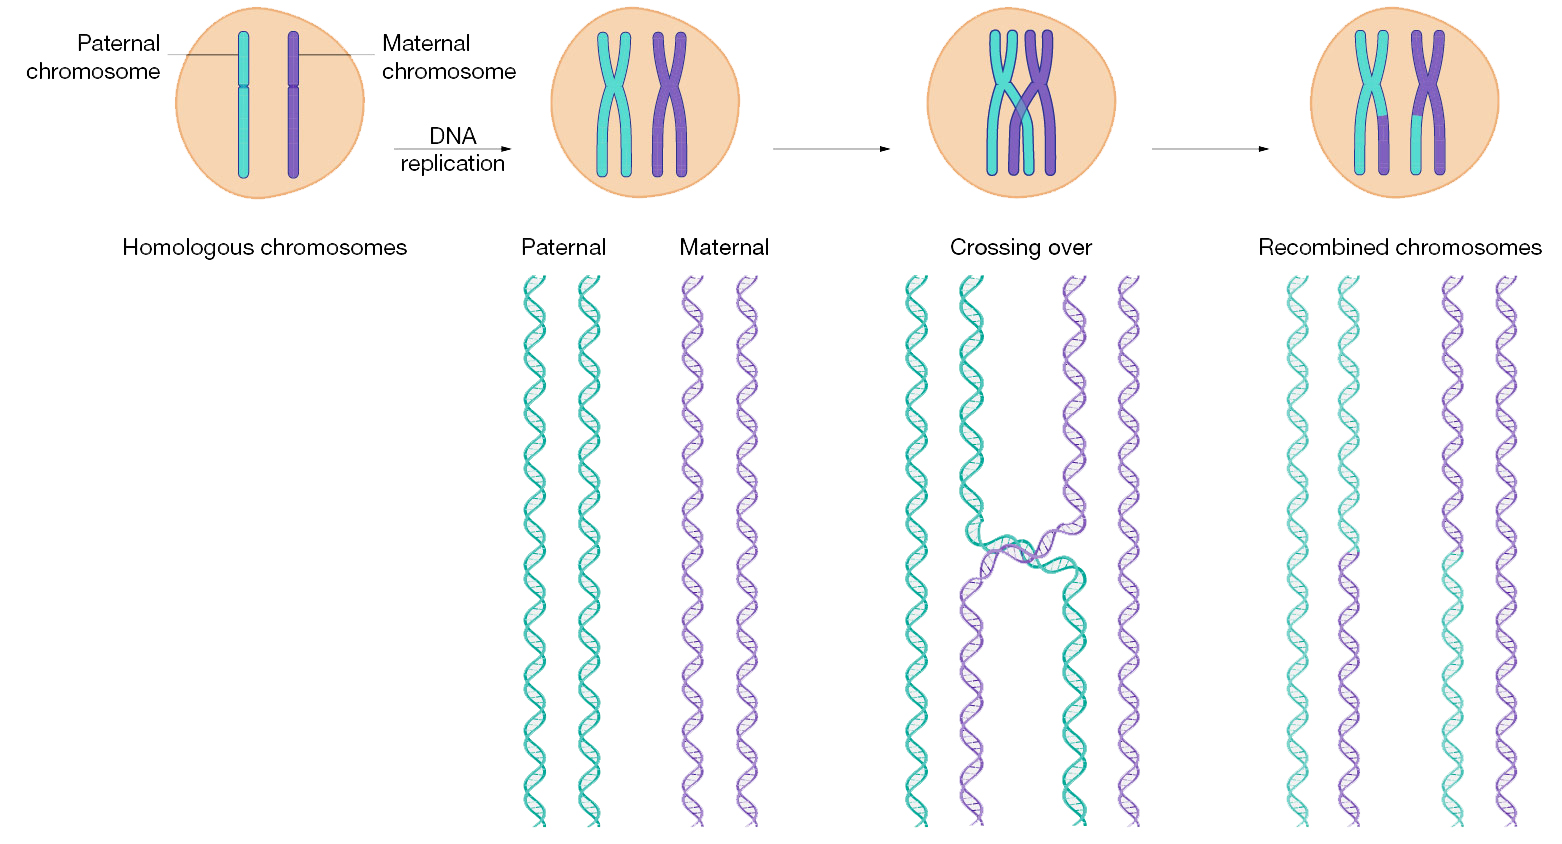
\includegraphics[width=375px]{hr.jpg}

  \caption{Homologous recombination between maternal and paternal chromosomes.}
  \label{fig:hr}
\end{figure}

However, a similar recombination process can also occur between repetitive DNA sequences that are similar but located in different (non-allelic) regions of the genome. This process is called non-allelic homologous recombination (NAHR). \\
It occurs between Low Copy Repeats (LCRs), also known as Segmental Duplications, that are DNA blocks of 10 to 400 kb in size with over
97\% identity between sequences \cite{burssed_mechanisms_2022}. NAHR can occur after a DSB during meiosis or mitosis when non-allelic copies of LCRs erroneously align due to their high level of sequence identity. This misalignment causes an unequal crossing over event generating genomic rearrangement in the daughter cells. 

\begin{figure}[h]

  \centering
    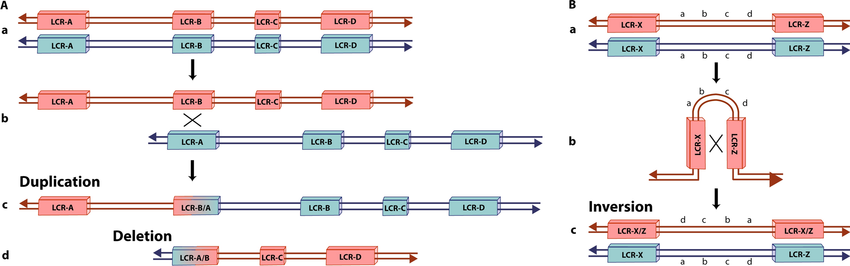
\includegraphics[width=400px]{nahr.png}

  \caption{Non-Allelic Homologous Recombination (NAHR) mechanism. A. NAHR leading to the formation of duplication and deletion: (a) Normal chromosome pairing and alignment of Low Copy Repeats (LCRs) in the same orientation. (b) A misalignment between LCRs due to their high level of sequence identity leads to an unequal crossing over event that can generate (c) a duplication and (d) a deletion. B NAHR leading to the formation of inversions: (a) Normal chromosome pairing and alignment of Low Copy Repeats (LCRs). LCR-X and LCR-Z present similar DNA sequences but in opposite orientations. (b) A misalignment between LCRs due to their high level of sequence identity leads to an unequal crossing over event that can generate (c) an inversion.}
  \label{fig:nahr}
\end{figure}

Through NAHR, regions located between segmental duplications or highly identical repeat sequences may be deleted, duplicated or inverted. Inversions can be formed by this process if the duplicated sequences are in inverted orientation with respect to each other, as Figure \ref{fig:nahr}B shows. Therefore, NAHR is considered the primary mechanism by which large (tens of kilobases) inversions are formed \cite{feuk_inversion_2010}. 

\section{Inversion in human disorders}

Many inversions traditionally detected in human karyotypes do not appear to have any phenotypic effects of clinical significance. This is the case of pericentric inversions (the inverted sequence includes the centromere) in chromosomes 1, 2, 3, 5, 9, 10 and 16. These mainly invert heterochromatic sequences and are frequently observed in cytogenetic analysis \cite{puig_human_2015}. However, not all inversions are harmless, and several diseases have been found to be occasionally caused by inversions, mostly due to direct disruption of one gene or alteration of its gene expression. These inversions appear de novo in patients or are inherited mutations restricted to a given family. \\
Since inversions are relatively rare events, and it is unlikely to have multiple patients with the same inversion, it is often problematic to assess whether the inversion present in the patient is actually associated with the phenotype. The exception is when the inversion breakpoint falls within or near a gene that has previously been associated with a disorder through other types of mutations. For recurrent inversions, the association between phenotype and genotype is more obvious, and a number of such loci have been described. One of the best-characterized disease-triggering recurrent inversions is linked to hemophilia A, an X-linked disorder caused by mutations in the factor VIII gene. A recurrent inversion has been found in approximately 43\% of patients.
Molecular characterization of the breakpoints indicates that the inversion is a result of intra-chromosomal homologous recombination, originating almost exclusively in male germ cells. This recurrent inversion spans approximately 400 kb and is mediated by two inverted segmental duplications, one of which is located in intron 22 of the factor VIII gene, with two other copies being located approximately 400 kb telomeric to the gene. Other examples where recurrent inversions have been shown to lead to a disease phenotype are the disruption of the idunorate 2-sulphatase gene in mucopolysaccharidosis type II (Hunter syndrome), and disruption of the emerin gene in Emery-Dreifuss muscular dystrophy \cite{feuk_inversion_2010}. \\
In addition to this, it was found that the presence of micro-inversions, defined as inversion in DNA shorter than 100 bp, can be linked to cancer, as shown by a study conducted in 2018 \cite{qu_micro-inversions_2018}. This study analyzed the distribution of micro-inversions among 24 chromosomes in four types of cancer (hepatocellular, lung, pancreatic and bladder), and found that the average count of micro-inversions per individual in the normal samples was lower than that of any type of cancer, showing that there is a high chance that micro-inversions may be associated with cancer development (see Figure \ref{fig:cancer}).

\begin{figure}[h]

  \centering
    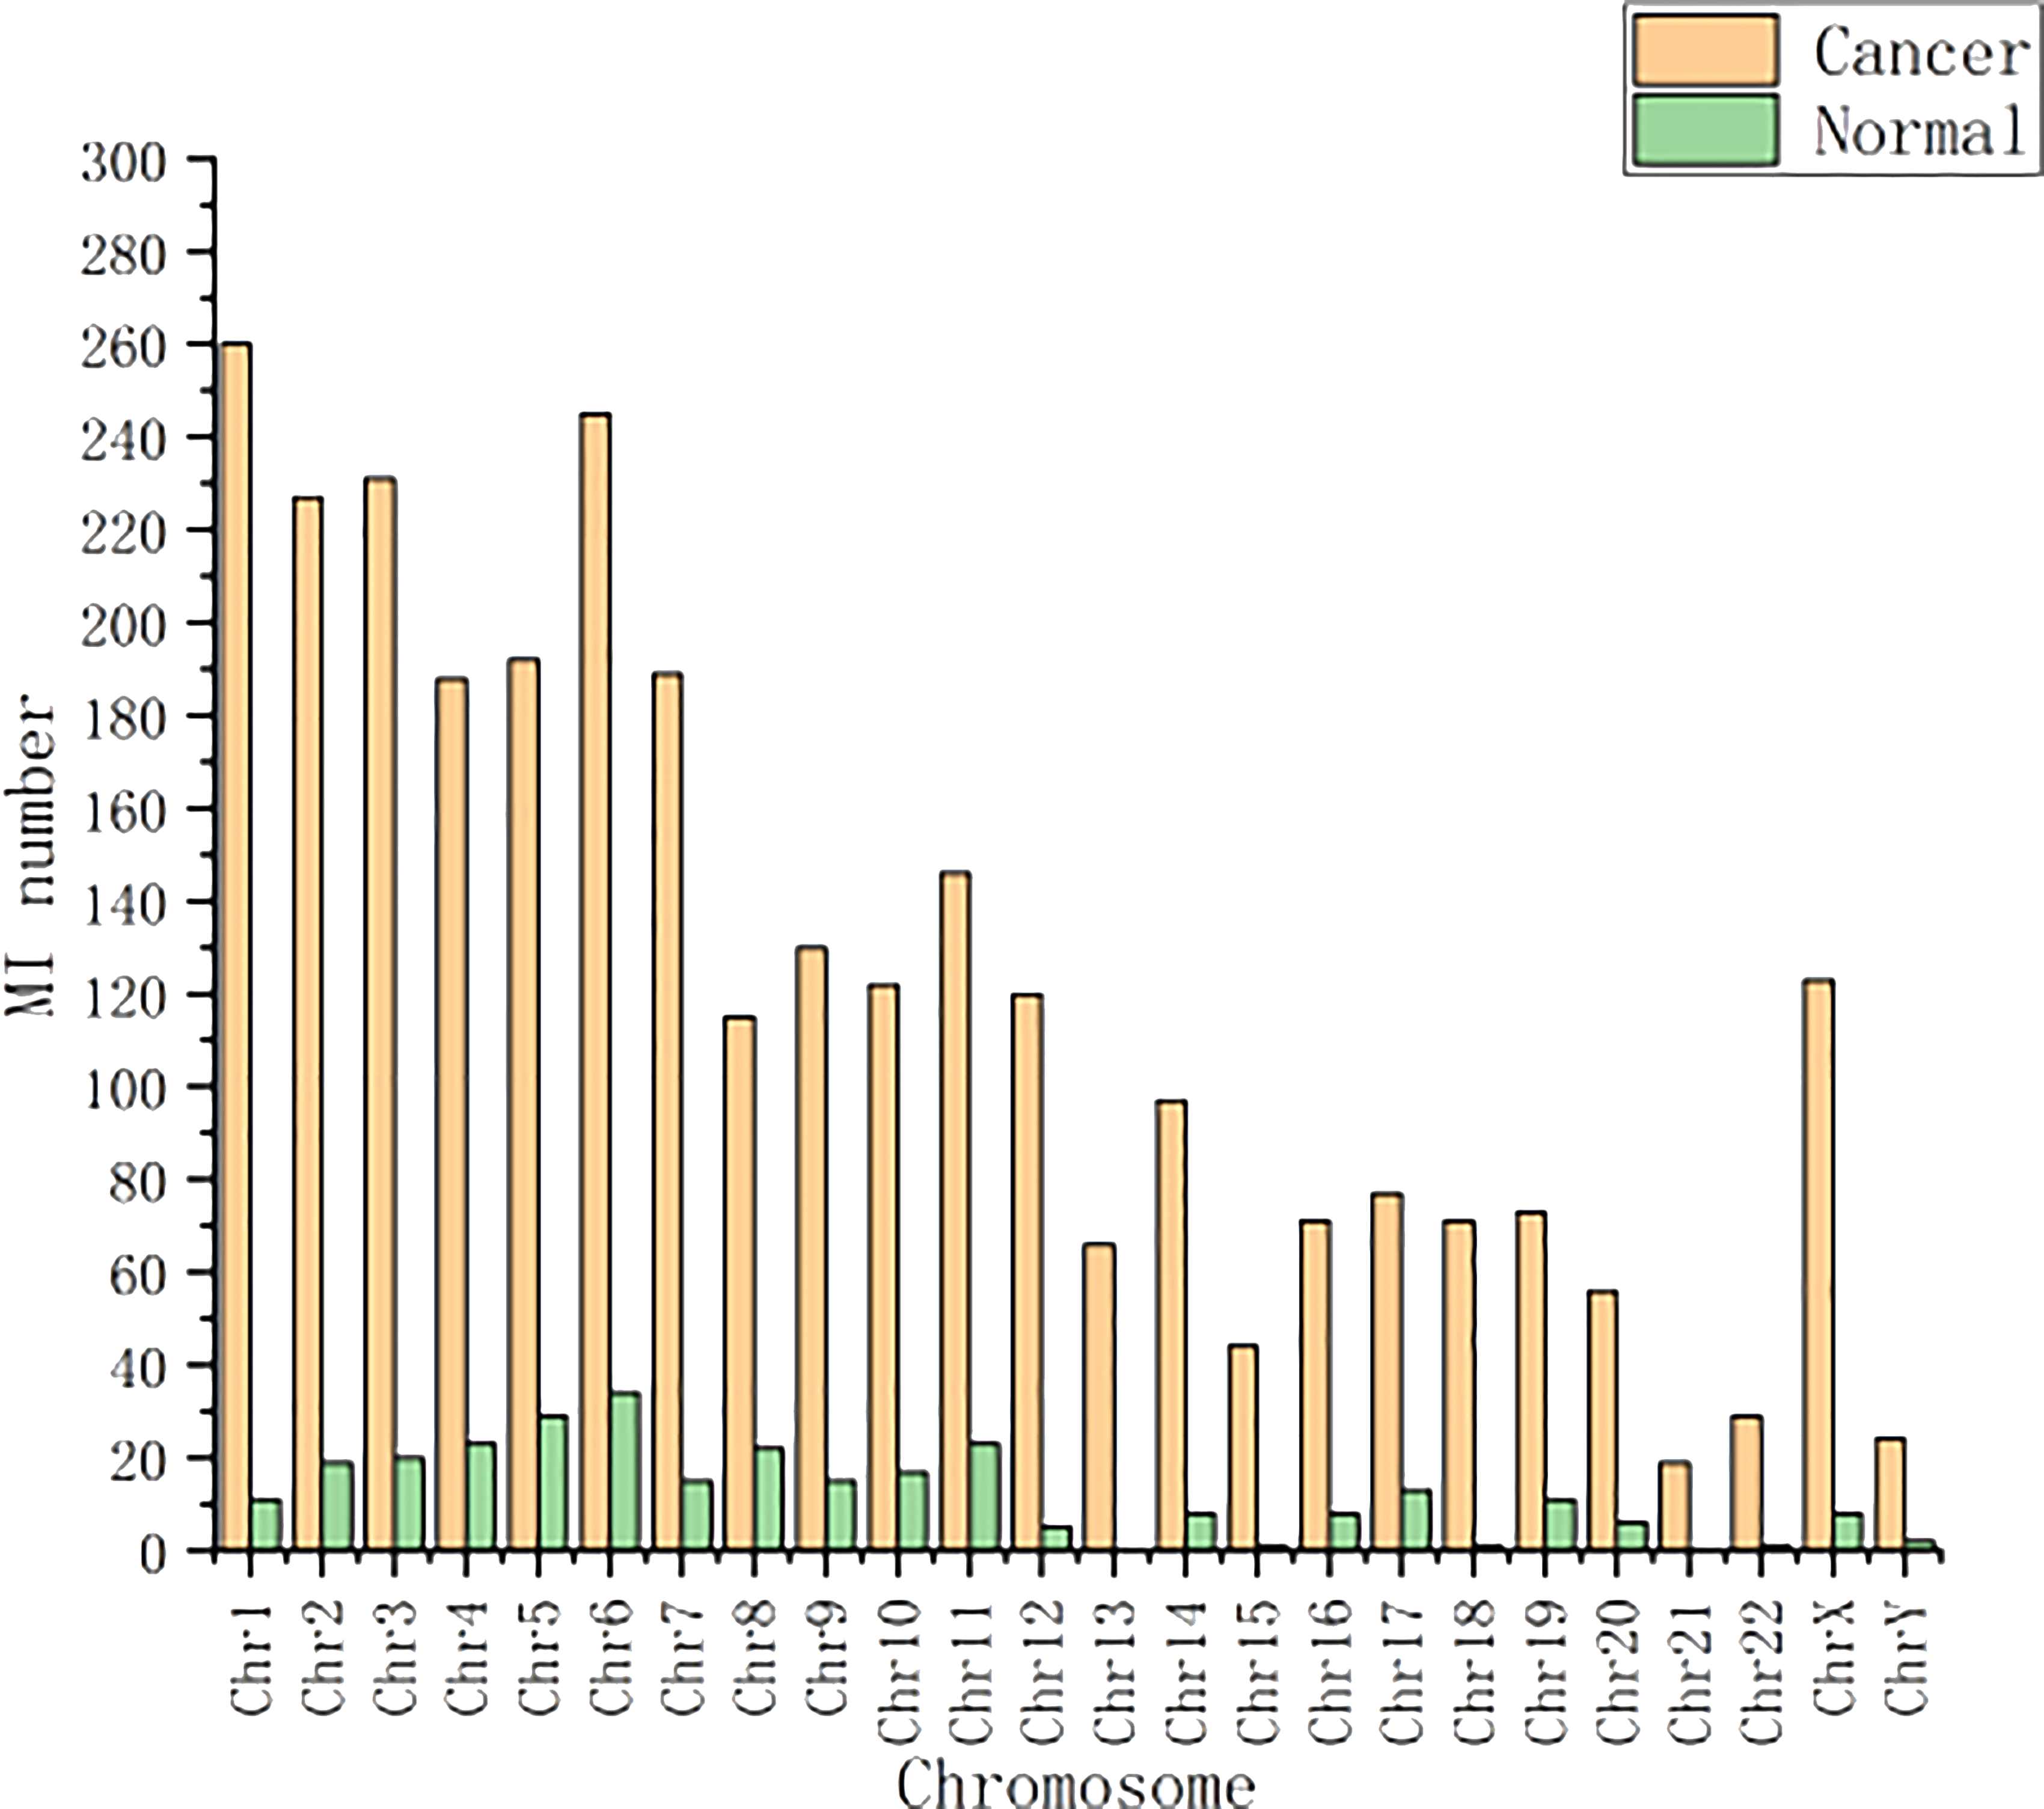
\includegraphics[width=250px]{cancer.png}

  \caption{Micro-inversion (MI) distribution among 24 chromosomes.  Average count of MIs per individual among the four types of cancer.}
  \label{fig:cancer}
\end{figure}
\newpage
\section{Knuth-Morris-Pratt Algorithm}

Knuth-Morris-Pratt \cite{knuth_fast_1977} (KMP) is the algorithm that will be used in this project to detect the position of inverted segments within the reference. It can be seen as an evolution of the naïve string-matching algorithm. In fact, given a text \textit{T} having length \textit{n} and a pattern \textit{P}, the naïve algorithm, for each possible starting position \textit{i}, where 0 \leq \textit{i} \leq \textit{n} - \( m \), compares the substring starting at position \textit{i} in the text with the pattern. If a mismatch is found, it moves to the next position. If all the characters match, it returns the occurrence of the pattern at index \textit{i}. \\
The idea behind the Knuth-Morris-Pratt algorithm is that, in case of mismatch, it is possible to perform a shift greater than 1, in order to avoid unnecessary comparisons. 

\subsection{LPS array}
KMP preprocesses the pattern by building an auxiliary array, the Longest Prefix Suffix (LPS) array. For each index \( i \) of the pattern \( P \), \( LPS[i] \) contains the length of the longest proper prefix of the substring \( P[:i] \) which is also a suffix of said substring. This array is the key to the algorithm’s efficiency. It helps in skipping characters that will certainly match, thus reducing the number of comparisons needed and ultimately speeding up the search process.  \\
The process of building the LPS array can be described as follows:

\begin{itemize}
\item Initialization: an array \( LPS[] \), of size equal to the length of the pattern is initialized with zeros. \( LPS[0] \) is set to 0 because there is no proper prefix for a single character. Two pointers are also initialized: \( i \), which iterates through the pattern, is set to 1, and \( j \), which will track the length of the previous longest proper prefix suffix, is set to 0.
\item Iteration over the pattern: each character at index \( i \) in the pattern is compared with the character at index \( j \) in the text. If \( P[i] == P[j] \), the current character in the pattern extends the longest proper prefix that is also a suffix, so both indexes \( i \) and \( j \) are incremented and \( LPS[i] = j\). Otherwise, if \( P[i] != P[j] \), the previously computed \( LPS[j-1] \) is checked to determine the next smaller prefix that could still match. If \( j == 0 \), there is no valid prefix to fall back to, so \( LPS[i] \) is set to 0 and \( i \) is incremented in order to move to the next character. 
\end{itemize}

The process continues until \( i\) reaches the length of the pattern.

\begin{figure}[h]

  \centering
    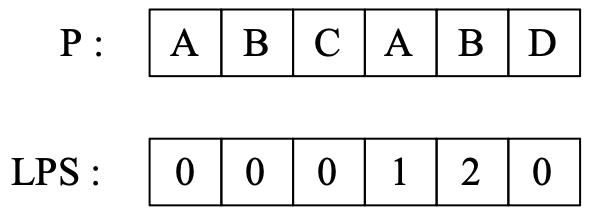
\includegraphics[width=250px]{lps.png}

  \caption{For the pattern \( P \) displayed in the figure, for the first three positions, \( LPS[i] \) equals to 0 because there is no proper prefix for "A", "AB" or "ABC" which is also a suffix. Moving on, \( LPS[3] \) is 1 because the proper prefix "A" of "ABCA" is also a suffix, \( LPS[4] \) is 2 because the proper prefix "AB" of "ABCAB" is also a suffix. For the last position, \( LPS[5] \) is, again, 0, since no proper prefix of "ABCABD" is also a suffix.}
  \label{fig:lps}
\end{figure}

\subsection{Pattern matching}

The KMP algorithm iterates through the text \( T \) and through the pattern \( P \), using two separate pointers. When a character in the reference matches a character in the pattern, both pointers are incremented to continue the comparison. 
When a mismatch is found at position  \( j \) in the reference and \( i \) characters of the pattern have already been matched, instead of restarting from the beginning of the pattern as it happens in the naïve algorithm, KMP consults \( LPS[i-1] \) in order to determine how many characters of the pattern can be skipped. Thus, the KMP algorithm performs pattern matching in $\mathcal{O}(n + m)$ time, where \( n \) is the length of the reference and \( m \) is the length of the pattern.

\begin{figure}[h]

  \centering
    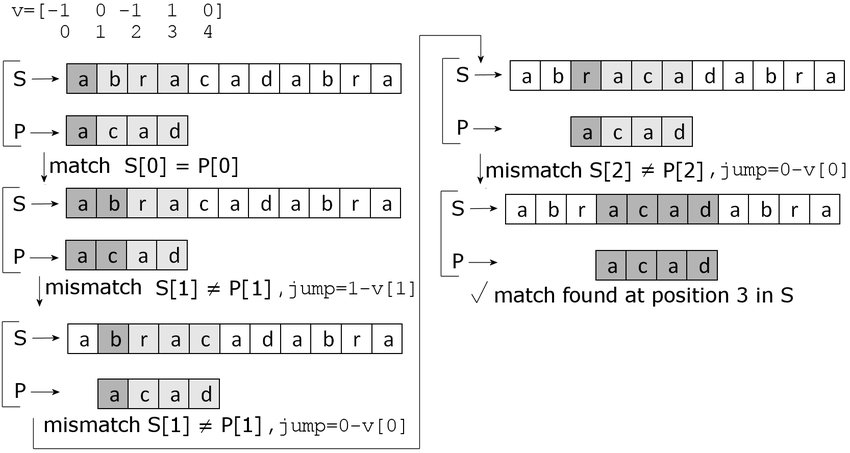
\includegraphics[width=300px]{kmp.jpeg}
    \caption{The KMP matching process for S = "abracadabra" and P = "acad".}
  \label{fig:kmp}
\end{figure}

Among other solutions, like the suffix array or the Boyer-Moore algorithm, the KMP algorithm was chosen for this project because it is more suitable in contexts with a very limited alphabet, such as DNA ({A, C, T, G}). Additionally, KMP performs well even when the length of the reference is large, unlike, for example, the suffix array method, which which can become less efficient in such cases due to its preprocessing requirements. This makes KMP the optimal choice for detecting inversions from long reads in the reference. 

\section{DNA sequencing}

In bioinformatics, DNA sequencing is the process of determining the sequence of nucleotides (As, Ts, Cs, and Gs) in a strand of DNA. A read is defined as a raw sequence generated by a sequencing machine\footnote{https://samtools.github.io/hts-specs/}. A read may consist of multiple segments. For sequencing data, reads are indexed in the order in which they are sequenced. Most next-generation sequencing technologies fragment the genome prior to sequencing, and each sequenced fragment produces a read. The length of the read and how many are produced will depend on fragment size and the type of technology used. As the fragments of DNA usually overlap, the reads can be pieced back together to reconstruct the genome. The length of the read is the number of bases that are read at one time, hence the number of letters that will appear in each read. In general, they can be divided into:

\begin{itemize}
\item \textbf{Short reads: } have lengths usually ranging from 50 to 300 base pairs. They are effective for applications aimed at counting the abundance of specific sequences, identifying variants within otherwise well-conserved sequences, or for profiling the expression of particular transcripts. Short-read sequencing is the best way to obtain high-depth, high-quality data at the lowest cost per base. On the other hand, short reads fail to generate a sufficient overlap between the DNA fragments. Overall, this means that it can be challenging to use them for sequencing highly complex, repetitive libraries, like the human genome. The dominant technologies in this field are Illumina’s platform and Thermo Fisher Scientific’s Ion Proton. However, multiple new sequencing technologies have surfacedin 2022, and have now been introduced to the market, helping to drive short-read sequencing costs even lower. These include instruments from Element Biosciences, Ultima Genomics, MGI, Singular Genomics and the PacBio acquired technology, Omniome\footnote{https://frontlinegenomics.com/long-read-sequencing-vs-short-read-sequencing/}. 
\item \textbf{Long reads: } have lengths usually ranging from 5000 to 50000 base pairs \cite{lee_error_2014}. They allow to identify complex SVs such as large insertions/deletions, inversions, repeats, duplications, and translocations. Long read NGS instruments have been on the market for the past decade but the lower yield, higher error rate, and higher costs of the instruments, have kept them from being more widely adopted. An additional downside is that the accuracy per read can be much lower than that of short-read sequencing. In the last decade, PacBio and Oxford Nanopore Technologies (ONT) have both been working to make long-read sequencing more accessible. Specifically, PacBio has improved the chemistry on their Sequel II instruments, enabling “HiFi sequencing” via circular consensus, which allows for sequencing of up to 15-20 kb pieces of DNA with error rate that are closer to short read sequencing.

\end{itemize}

Sequencing data are the main input of several bioinformatics algorithms. The algorithm described in this work uses long read sequencing data. Indeed, due to their length, they are suited to detect enough long inversions. 

\section{FASTA format}

FASTA is a text-based format used in bioinformatics to represent DNA sequences, in which base pairs are represented using a single-letter code from the alphabet \(\Sigma = \{A, C, G, T\}\),  where each letter corresponds to the initial of one of the four nitrous bases that make up the DNA. The format also allows for sequence names and comments to precede the sequences. As detailed in Chapter 4 below, FASTA will be used in this project to represent both the reference sequence and the target, which is a long read of the reference. A FASTA sequence begins with a single-line identifier description, followed by lines of DNA sequence data. The identifier description line is distinguished from the sequence data by a greater-than ('\( \textgreater \)') symbol in the first column. The word following the "\( \textgreater \)" symbol is the identifier of the sequence, and the rest of the line is an optional description separated from the identifier by a white space or tab. The sequence data starts on the next line following the text line and ends at the appearance of another line starting with a "\( \textgreater \)", which signals the start of another sequence. The extension of this format is usually \texttt{.fa}. 

\begin{example}
  This is an example of a portion of a FASTA file that contains two nucleotide sequences:
\begin{verbatim}
>NC_045512.2 
ATTAAAGGTTTATACCTTCCCAGGTAACAAACCAACCAACTTTCGATCTCTTGTAGATCT
GTTCTCTAAACGAACTTTAAAATCTGTGTGGCTGTCACTCGGCTGCATGCTTAGTGCACT
>OL700521.1 
GTTCTCTAAACGAACTTTAAAATCTGTGTGGCTGTCACTCGGCTGCATGCTTAGTGCACT
CACGCAGTATAATTAATAACTAATTACTGTCGTTGACAGGACACGAGTAACTCGTCTATC
\end{verbatim}
\end{example}





\chapter{Algorithm}
\newtheorem{theorem}{Theorem}
\renewcommand\proofname{Proof}
\begin{algorithm}
\caption{Check For Inversions Using Sample-Specific Strings}
\hspace*{\algorithmicindent} \textbf{Input: } \text{indexes}: list of integers, \text{lengths}: list of integers, \text{sample\_specific\_strings}: list of strings, \text{target}: string, \text{reference}: string \\
\hspace*{\algorithmicindent} \textbf{Output: } list of reverted sequences found in \text{target}

\begin{algorithmic}[1]

\STATE \text{reverted} $\gets$ [ ]

\FOR{$i \gets 1$ \TO $\text{sample\_specific\_strings.length} - 1$}
    \STATE $j \gets \text{indexes}[i]$
    \STATE $k \gets \text{indexes}[i + 1]$
    
    \IF{$j == -1$ \OR $k == -1$}
        \STATE \textbf{CONTINUE}
    \ENDIF
 
    \STATE \text{middle} $\gets$ \text{target}$[j + \text{lengths}[i]:k]$
    \IF{$\text{middle} == \emptyset$}
        \STATE \textbf{CONTINUE}
    \ENDIF

    \STATE \text{middle} $\gets$ \textbf{REVERT\_AND\_COMPLEMENT}(\text{middle})
    \STATE (\text{found}, \text{start}) $\gets$ \textbf{CHECK\_SUBSTRING}(\text{reference}, \text{middle})

    \IF{\text{found}}
        \STATE \text{left\_increment} $\gets 1$
        \WHILE{$\text{left\_increment} \leq \text{lengths}[i]$ \AND $(j + \text{lengths}[i] - \text{left\_increment}) \geq 0$ \AND \text{target}$[j + \text{lengths}[i] - \text{left\_increment}] == \textbf{REVERT\_AND\_COMPLEMENT}(\text{reference}[\text{start} + \text{middle.length} + \text{left\_increment} - 1])$}
            \STATE \text{left\_increment} $\gets \text{left\_increment} + 1$ 
        \ENDWHILE
        \STATE \text{left\_breakpoint} $\gets$ \text{target}$[j + \text{lengths}[i] - \text{left\_increment}: j + \text{lengths}[i] - \text{left\_increment} + 2]$

        \STATE \text{right\_increment} $\gets 0$
        \WHILE{$\text{right\_increment} < (\text{reference.length} - \text{start} - \text{middle.length}$ \AND $(k + \text{right\_increment}) < \text{target.length}$ \AND \text{target}$[k + \text{right\_increment}] == \textbf{REVERT\_AND\_COMPLEMENT}(\text{reference}[\text{start} - 1 - \text{right\_increment}])$}
            \STATE \text{right\_increment} $\gets \text{right\_increment} + 1$
        \ENDWHILE
        \STATE \text{right\_breakpoint} $\gets$ \text{target}$[k + \text{right\_increment} - 1: k + \text{right\_increment} + 1]$

        \STATE \textbf{PRINT} ``\textit{left\_breakpoint} and \textit{right\_breakpoint} are breakpoints of an inversion''

        \STATE \text{inversion} $\gets$ \text{target}$[j + \text{lengths}[i] - \text{left\_increment} + 1: k + \text{right\_increment}]$
        \STATE \textbf{APPEND} \text{reverted} $\gets$ \text{inversion}
    \ENDIF
\ENDFOR
\RETURN \text{reverted}
\end{algorithmic}
\end{algorithm}




\begin{algorithm}
\caption{Revert and Complement DNA Sequence}
\hspace*{\algorithmicindent} \textbf{Input: } DNA sequence: string \\
\hspace*{\algorithmicindent} \textbf{Output: } reverted and complemented sequence: string
\begin{algorithmic}[1]


\STATE $\text{complements} \gets \{ 'A': 'T', 'C': 'G', 'G': 'C', 'T': 'A' \}$
\STATE $\text{reverted\_complement} \gets \varepsilon$

\FOR{$i \gets \text{sequence.length} - 1$ \TO $0$}
    \STATE $base \gets \text{sequence}[i]$
    \STATE $complement \gets \text{complements}[base]$
    \STATE $\textbf{APPEND} \text{ reverted\_complement} \gets complement$
\ENDFOR

\RETURN $\text{reverted\_complement}$
\end{algorithmic}
\end{algorithm}


\begin{algorithm}
\caption{Knuth-Morris-Pratt Prefix Function}
\hspace*{\algorithmicindent} \textbf{Input:} pattern: string \\
\hspace*{\algorithmicindent} \textbf{Output:} LPS array: list of integers

\begin{algorithmic}[1]
\STATE $m \gets \text{length of pattern}$
\STATE $\text{lps} \gets [0] * m$ 
\STATE $j \gets 0$ 
\STATE $i \gets 1$
\WHILE{$i < m$}
    \IF{$\text{pattern}[i] == \text{pattern}[j]$}
        \STATE $j \gets j + 1$
        \STATE $\text{lps}[i] \gets j$
        \STATE $i \gets i + 1$
    \ELSE
        \IF{$j \neq 0$}
            \STATE $j \gets lps[j - 1]$
        \ELSE
            \STATE $lps[i] \gets 0$
            \STATE $i \gets i + 1$
        \ENDIF
    \ENDIF
\ENDWHILE
\RETURN $\text{lps}$
\end{algorithmic}
\end{algorithm}

\begin{algorithm}
\caption{Check Substring Using Knuth-Morris-Pratt}
\hspace*{\algorithmicindent} \textbf{Input:} reference: string, string: string \\
\hspace*{\algorithmicindent} \textbf{Output:} Tuple of boolean (True if string is a substring of reference) and integer (starting index if found, -1 otherwise)

\begin{algorithmic}[1]
\STATE $n \gets \text{length of reference}$
\STATE $m \gets \text{length of string}$
\STATE $\text{lps} \gets \text{KMP-Prefix/Function}(\text{string})$

\STATE $i \gets 0$ 
\STATE $j \gets 0$ 

\WHILE{$i < n$}
    \IF{$\text{string}[j] == \text{reference}[i]$}
        \STATE $i \gets i + 1$
        \STATE $j \gets j + 1$
    \ENDIF

    \IF{$j == m$}
        \RETURN $(\text{True}, i - j)$ 
    \ELSIF{$i < n$ \AND $\text{string}[j] \neq \text{reference}[i]$}
        \IF{$j \neq 0$}
            \STATE $j \gets \text{lps}[j - 1]$
        \ELSE
            \STATE $i \gets i + 1$
        \ENDIF
    \ENDIF
\ENDWHILE
\RETURN $(\text{False}, -1)$ 
\end{algorithmic}
\end{algorithm}




\section{Algorithm Overview}

The algorithm's primary objective is to detect reverted sequences within a target DNA sequence, which are characterized by segments that have been inverted and complemented relative to a reference DNA sequence. \\
It uses sample-specific strings as possible anchors of an inverted portion occurring in the target. The definition of sample-specific string is as follows:

\begin{definition}[Sample-specific string]
A sample-specific string S is a string that occurs in the target DNA string T, does not occur in the reference DNA string R, and for every string S' which is a substring of S, S' occurs in the reference string R. 
\label{thm:sample_specific}
\end{definition} 
The key components of the algorithm are:

\begin{itemize}
    \item Target Sequence: the DNA sequence in which the algorithm looks for reverted sequences. It is a long read extracted from the reference sequence;
    \item Reference Sequence: the DNA sequence used as a baseline to identify reverted sequences in the target;
    \item Sample-specific strings: see Definition \ref{thm:sample_specific}. They expected to appear in order within the target sequence;
\end{itemize}




\section{High-Level Explanation}

This algorithm is structured in a way that involves different phases, detailed as follows:

\begin{itemize}
    \item \textbf{Setup: } in this phase the working environment is set up, and relevant data structures are prepared in order to store relevant results. Given a target sequence \( S \) and a reference sequence \( R \), let \( I = \{ i_1, i_2, \dots , i_n \} \) denote the list of indexes where sample-specific strings occur in \( S \), and let \( L = \{ l_1, l_2, \dots , l_n \} \) be the list of their corresponding lengths. Additionally, an empty list, \( reverted \), is initialized to store any detected inverted sequences.
    \item \textbf{Iteration through sample-specific strings: } the algorithm focuses on the prime candidate for detecting inversions, which is the segment that lies between a couple of sample-specific strings. Therefore, the core of the algorithm involves iterating through each  pair of adjacent sample-specific strings.  It confronts every pair \( (x, y) \) of sample-specific strings within the range, where \( x = S[i_j : i_j + l_j] \) and \( y = S[i_{j+1} : i_{j+1} + l_{j+1}] \), and extracts the segment \( m \) that lies exactly in the middle of the two sample-specific strings \( x \) and \( y \). More precisely, \( m = S[i_j + l_j : i_{j+1}] \). The extracted segment \( m \) represents the region that could potentially be the inversion.
    \item \textbf{Reversing and Complementing: } when handling genomic data, an inversion is not just a reversal of the nucleotide sequence, but it also involves the complementing of bases, as seen on Chapter 2. After extracting the segment in the middle \( m \), its reverse complement \( m_r \) can be easily obtained: first, the bases in \( m \) are reversed, then each base is replaced with its complement. The segment \( m_r \) is the transformed version of \( m \) that allows the algorithm to search for inverted regions in \( R \). 
    \item \textbf{Search for the Reverse Complement in the Reference String: } the logic behind this step is that if \( m \) is actually an inverted segment, this means that its reverse and complement \( m_r \) can be found within the reference \( R \), since \( R \) represents the original, non-inverted version of the sequence. To efficiently locate \( m_r \) in \( R \), the algorithm uses the Knuth-Morris-Pratt (KMP) algorithm, detailed in Chapter 2. This method is used in combination with a prefix function, the longest prefix suffix array (LPS) that avoids unnecessary character comparisons. It preprocesses the pattern \( m_r \), creating an array that stores the lengths of the longest prefixes of the pattern that are also suffixes. When a mismatch occurs, the algorithm uses this information to skip ahead in the pattern, making the whole process more efficient. If \( m_r \) is found in \( R \), the starting index \( s \) of the occurrence of \( m_r \) in \( R \) is stored for further analysis. 
    \item \textbf{Identification of Breakpoints: } the identifications of breakpoints is essential to precisely locate the boundaries of the inversion within the target sequence \( S \). So, if the reverse complement \( m_r \) is found in \( R \), the algorithm proceeds to identify the inversion breakpoints, that define the boundaries of the inverted segment in \( S \). The breakpoints are determined by comparing characters from \( S \) and \( R \) in two stages:
    \begin{itemize}
    	\item \textbf{Left Breakpoint Identification: } starting from the last character of the first sample-specific string \( x \) in \( S \), that corresponds to \( S[i_j + l_j] \) and the first character immediately following \( m_r \) in \( R \), which is \( R[s + m_r .length] \), the algorithm compares corresponding characters from \( S \) and the reverse complement of \( R \). This comparison continues backward in \( S \) and forward in \( R \) until a mismatch occurs. At this point, the final position in \( S \) is marked as left breakpoint.
    	\item \textbf{Right Breakpoint Identification: } the right breakpoint is determined symmetrically. The comparison starts from the first character of the second sample-specific string \( y \) in \( S \), \( S[i_{j+1}] \), and the character immediately preceding \( m_r \) in \( R \), \( R[s - 1] \), and the search proceeds forward in \( S \) and backward in \( R \) until a mismatch is found, marking the right breakpoint in \( S \). 
    \end{itemize}
\end{itemize}

\section{Conditions for Proper Functioning}

The correctness of this algorithm is ensured if the middle segment extracted from the target is sufficiently long to ensure its uniqueness within the reference sequence. This  is crucial because if the middle segment is too short, it might match multiple locations within the reference sequence, leading to potential misalignment. This  can result in the algorithm identifying incorrect breakpoints or even falsely identifying an inversion that does not actually exist, hence a false positive. \\
In addition to this, for the algorithm to function properly, the target sequence, and particularly the middle segment, must be free of errors or mutations. In fact, even a single error within the middle segment can disrupt the transformation process, where the segment is reversed and complemented. As a result, the transformed segment may not match the expected part of the reference sequence, leading to false negatives where actual inversions are missed. 
\section{Edge Cases}
An important edge case to consider occurs when two sample-specific strings appear consecutively without any intervening characters in the target string. In this scenario, the middle segment will be an empty string. This happens because there are no characters between the end of the first sample-specific string and the beginning of the second one. For example:
\begin{itemize}
    \item \textbf{Sample-specific strings: } 'S1', 'S2'
    \item \textbf{Target string: }  '\dots S1S2\dots'
\end{itemize}

In this case the starting index of 'S1' is \textit{j} and the starting index of 'S2' is \textit{k}, making the middle segment target[j + S1.length : k], which evaluates to an empty string.

\section{Proof of Correctness}

Now that the algorithm has been explained in detail, the proof of its correctness will be provided. \\
Let \( S = xyz \) be a string, where \( x \), \( y \), and \( z \) are substrings of \( S \): Let also \(y^r \) be the reversal of \( y \), the aim is to demonstrate that it is possible to reconstruct the sequence \( S' = z^r y^r x^r \), where the superscript '\( r \)' indicates the reversal of a string. For the sake of simplicity, the complement will be ignored. The proof will be made using mathematical induction. 

\begin{figure}[h]

  \centering
    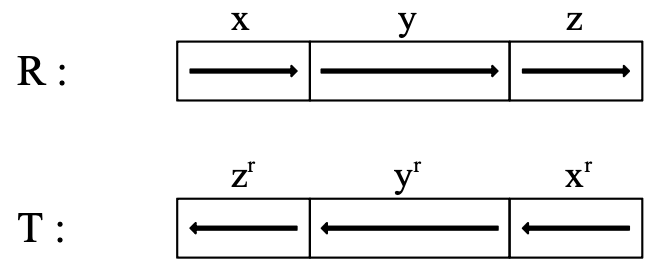
\includegraphics[width=300px]{rev.png}

  \caption{\( R \) represents the reference string, that in the following demonstration will be referred as \( S \), and \( T \) is the target where the inversion is found, that will be later referred as \( S' \)}
  \label{fig:rev}

\end{figure}

\begin{theorem}
    For any string \( S = xyz \), where \( x \), \( y \), \( z \) are substrings of \( S \), given \(y^r \), reversal of \(y\), it is possible to reconstruct the sequence \( S' = z^r y^r x^r \). 
\end{theorem}
\begin{proof}
\\ 
\textbf{Base case: } \|\( y \)\| = 1 \\
\\ Let \( \| y \| = 1 \), meaning \( y \) only consists of a single character '\( a \)'. In this trivial case, \( S = xaz \), and \(y^r \) = \( a \). Hence, the string \( S' = z^r y^r x^r \) can be reconstructed as follows: 
\begin{enumerate}
\item Reverse \( z \) to obtain \( z^r \);
\item Append \( y^r \), which is simply '\( a \)';
\item Append the reversal of \( x \), which is \( x^r \).
\end{enumerate}
The resulting sequence \( S' \) is \(z^r a x^r \), equivalent to \( S' = z^r y^r x^r \) when \|\( y \)\| = 1. \\
\\ \textbf{Inductive step: } \( \| y \| > 1 \) \\

\\ Assume that for some \( k > 1 \), it is possible to reconstruct \( S' = z^r y^r x^r \) when \( \| y \| = k \) (inductive hypothesis). It will be proven that this reconstruction is also possible when \( \| y \| = k + 1 \). 

Let \( y = a_1 a_2 \dots a_k a_{k+1} \), where each \( a_i \) is a single character. Thus, \( y^r = a_{k+1} a_k \dots a_2 a_1 \). According to the inductive hypothesis, it is possible to reconstruct \( S' = z^r (a_1 a_2 \dots a_k)^r x^r \). In order to obtain \( S' = z^r y^r x^r \) for \( \| y \| = k + 1 \), the following steps are necessary:
\begin{enumerate}
    \item Start with \( z^r (a_k \dots a_2 a_1) x^r \);
    \item Insert \( a_{k+1} \) before \( a_k \dots a_2 a_1 \);
\end{enumerate}
The result is \( z^r (a_1 a_2 \dots a_k a_{k+1})^r x^r \), which corresponds to \( S' = z^r y^r x^r \) for \( \| y \| = k + 1 \).
\end{proof}

\section{Time and Space Complexity}
Now, the time and space complexity of the algorithm will be analyzed. \\
Starting with the first one, during the initialization phase, the necessary parameters are set up, and the list to store the reverted sequences is initialized. These steps are performed in constant time, hence $\mathcal{O}(1)$. \\

In the iteration phase, each pair of sample-specific strings is processed. Let \( n \) denote the total number of sample-specific strings, each interaction involves the extraction of the segment \( m \) between two adjacent sample-specifics strings. This step is repeated for each pair, and extracting the segment takes time proportional to its average length $\bar{m}$, so the overall time complexity of this phase is $\mathcal{O}(n \cdot \bar{m} )$. \\

In the following phase, the segment in the middle is transformed by reverting its characters and complementing each base. This operation takes $\mathcal{O}( \bar{m})$ time per iteration, so the overall time complexity of this phase is, just like the previous one, $\mathcal{O}(n \cdot \bar{m} )$. \\

For the search in the reference string, the Knuth-Morris-Pratt algorithm is used to locate the transformed segment \( m_r \) within the reference \( R \). First, the LPS array is constructed. The array is initialized of size \( m \), where \( m \) is the length of the pattern. Keeping in mind that this data can vary when multiple inversions having different lengths are found during the whole computation, the actual value to analyze is the average length \( \bar{m} \).  Then, the algorithm iterates through the pattern and the LPS array is filled based on the comparison of the characters in the pattern. Each character is processed at most twice: once when a match is found, and again if a mismatch occurs (when the pointer \( j \) is reset based on the LPS array). Therefore, the time complexity required for the LPS computation is $\mathcal{O}(\bar{m})$, hence linear. \\
Once built the LPS array, the actual search of the substring begins, iterating over the characters in the reference string while using the information in the LPS array in order to skip unnecessary comparisons. Each character in the reference string is processed at most once. Additionally, the character comparisons are skipped according to the values in the LPS array. Therefore, said \( r \) the length of the reference, the time complexity of the search is  $r + \mathcal{O}(\bar{m})$, which also makes the total time complexity of the whole phase. \\

In the last phase, the algorithm identifies the left and right breakpoints, which requires comparing characters in both target and reference sequences. Considering the search of the left breakpoint, where the algorithm starts at the last character of the first sample-specific string in the target and the character immediately following the segment in the middle segment extracted in the reference, the number of comparisons performed depends on the length of the first sample-specific string. Said \( s \) such length, in the worst case scenario, the algorithm compares \( s \) characters. The process is the same for the right breakpoint, but the length of the second sample-specific string may differ. Therefore, the time complexity must be proportional to the average length of the sample-specific strings, that will be referred as $\bar{s}$. Since the algorithm iterates over \( n \) sample-specific strings, the total time complexity of this phase is $\mathcal{O}(n \cdot \bar{s} )$. \\

The overall time complexity is determined combining all the phases. Therefore, it can be expressed as $\mathcal{O}(n \cdot \bar{m} + n \cdot \bar{m} + r + \bar{m} + n \cdot \bar{s})$ and summarized as $\mathcal{O}(n \cdot \bar{m} + r + \bar{m} + n \cdot \bar{s})$. In this scenario, $\bar{m}$ is considerably smaller than the reference length  \( r \), and the same can be said for the average length of the sample specific strings \( \bar{s} \). So, the dominant terms that actually determine the total time complexity of the algorithm are $n \cdot \bar{m}$ and \( s \). Consequently, the result is $\mathcal{O}(r + n \cdot \bar{m} )$. \\


Regarding space complexity, the algorithm requires $\mathcal{O}(n \cdot \bar{m} )$ space to store the list of reverted sequences. Additionally, the LPS array used in the Knuth-Morris-Pratt algorithm demands $\mathcal{O}(\bar{m} )$ space for each segment processed and temporarily stored during the search phase. Temporary variables for indexing and counters occupy $\mathcal{O}(1)$ space. Although the middle segments are not stored long-term, the memory requirements are still significant due to the storage of reverted sequences. Therefore, the overall space complexity of the algorithm is $\mathcal{O}(n \cdot \bar{m} )$.



















































\chapter{Experimentation}
\section{Implementation}
The practical experimentation was carried out using the SVDSS \cite{denti_svdss_2023} tool on a Linux Ubuntu virtual machine installed on MacOS, in order to detect the sample-specific strings. It requires two input files: the reference and the target, both in \texttt{FASTA} format. A \texttt{Python} script, \texttt{input\_generator.py}, was used to generate mock examples. It creates a random DNA sequence and a modified copy with one or more inversions, producing two output files: \texttt{reference.fa} and \texttt{target.fa}. Numerous tests were conducted with strings of varying lengths in order to verify that the algorithm was functioning properly.

The tool is available at a public Git repository\footnote{https://github.com/Parsoa/SVDSS} on GitHub. Once the SVDSS binary file \texttt{SVDSS\_linux\_x86-64} is downloaded, the file permissions must be modified using the shell to make it executable, with the following command: 

\begin{verbatim}
chmod +x SVDSS_linux_x86-64
\end{verbatim}

Next, the reference file must be indexed, generating the output file \texttt{index.fmd} using the following command: 

\begin{verbatim}
./SVDSS_linux_x86-64 index --reference reference.fa --index index.fmd
\end{verbatim}

The final step is to run the command to generate the \texttt{specifics.txt} file containing all the sample-specific strings detected and related data: 

\begin{verbatim}
./SVDSS_linux_x86-64 search --index index.fmd --fastx target.fa  
\end{verbatim}

\begin{verbatim}
--bsize 10 > specifics.txt
\end{verbatim}

The file \texttt{specifics.txt}, which is needed by the code implementing the algorithm described in Chapter 3, has the following structure, as generated by a random test:

\begin{verbatim}
T       90      19      0
*       240     19      0
*       492     16      0
*       625     15      0
\end{verbatim}

The fields in the file are as follows:
\begin{itemize}
\item The target sequence where the sample-specific strings are detected in comparison to the reference. If the sample-specific strings are detected in the same target as the previous row, the symbol "\texttt{*}" is displayed;
\item The index where the sample-specific string starts;
\item The length of the sample-specific string;
\item An additional field that will not be analyzed. 
\end{itemize}

In this case the tool found four sample-specific strings within a single target, at indexes 90, 240, 492 and 625 and having length 19, 19, 16 and 15. \\
This file is given in input to the actual \texttt{Python} implementation of the algorithm, together with the \texttt{reference.fa} and \texttt{target.fa} \texttt{FASTA} files generated by \texttt{input\_generator.py}. A function \texttt{read\_fasta} reads \texttt{reference.fa} and \texttt{target.fa} and converts them into two strings, in order to be better analyzed. Another function \texttt{build\_sample\_specific\_data} takes  \texttt{target.fa} and the generated file  \texttt{specifics.txt} and builds three lists: one of indexes, one of lengths, and one of sample-specific strings found in the target. This information will be needed by the function  \texttt{check\_reverted\_sample\_specific} that is the actual implementation of the algorithm. This function implements the main algorithm for detecting inversion breakpoints by analyzing the sample-specific strings.\\
The user will choose the boundaries, which are the indexes of the first and the last sample-specific strings that will be taken into consideration. This will help narrow down the analysis to a smaller and more manageable subset of sample-specific strings, and will be extremely helpful in the cases where regions with a high chance of having inversions are known. \\
In output are given the inverted sequences, the breakpoints of the inversions and the time taken to execute the program, that will be needed in the following section to analyze the results. \\
All the described \texttt{Python} files are available at a public Git repository\footnote{https://github.com/silviacambiago/bachelor-thesis} on GitHub.

\section{Results}

The experimentation was conducted using various reference lengths and a target of fixed length, 50000 bp, making sure to simulate an actual long read. The reference lengths considered were 50000 bp, 100000 bp, 1000000 bp, and 10000000 bp. Since time complexity also depends on the number of inversions and their lengths, the generated samples contained 2, 4 and 6 inversions, both short or long. The first ones were, on average, 250 bp, while the latter ones 6500 bp on average. \\

\subsection{No segmental duplications}
This data was collected making 10 experimentations for each combination of reference lengths - number of inversions - length of inversions, and calculating the average time measured in seconds, using the \texttt{time} library provided by \texttt{Python}. For this first set of experimentations, the samples have no segmental duplications. Table \ref{res} sums up the results:

\renewcommand{\arraystretch}{1.2} 

 \begin{table}[h!]
\centering
\resizebox{\textwidth}{!}{%
\begin{tabular}{l c cc cc cc}
\toprule
\multirow{2}{*}{\textbf{Reference}} & \multirow{2}{*}{\textbf{Target}} & \multicolumn{2}{c}{\textbf{2 Inversions}} & \multicolumn{2}{c}{\textbf{4 Inversions}} & \multicolumn{2}{c}{\textbf{6 Inversions}} \\
\cmidrule(lr){3-4} \cmidrule(lr){5-6} \cmidrule(lr){7-8}
                                    &                                   & \textbf{Short} & \textbf{Long} & \textbf{Short} & \textbf{Long} & \textbf{Short} & \textbf{Long} \\ 
\midrule
50000       & 50000 & 0.0188 & 0.0260 & 0.0407 & 0.0459 & 0.0721 & 0.0758 \\
100000      & 50000 & 0.0353 & 0.0400 & 0.0828 & 0.0934 & 0.1336 & 0.1396 \\
1000000     & 50000 & 0.3009 & 0.3029 & 0.7305 & 0.8364 & 1.2190 & 1.2535 \\
10000000    & 50000 & 2.9765 & 3.0082 & 7.3140 & 7.6067 & 11.8296 & 12.1238 \\
\bottomrule
\end{tabular}%
}
\caption{Execution times for various reference lengths and target lengths with different numbers of short and long inversions.}
\label{res}
\end{table}

These data demonstrates that the execution time increases dramatically with larger reference lengths, making it practically the dominant factor when it comes to complexity, as shown by the graph in Figure \ref{fig:refgraph}. For example, for 2 short inversions, the time rose from 0.0188 \( s \) at \( r \) = 50000 to 2.9765 \textit{s} at \( r \) = 10000000, highlighting the substantial contribution of \( r \) to the overall complexity. \\

\begin{figure}[h]

  \centering
    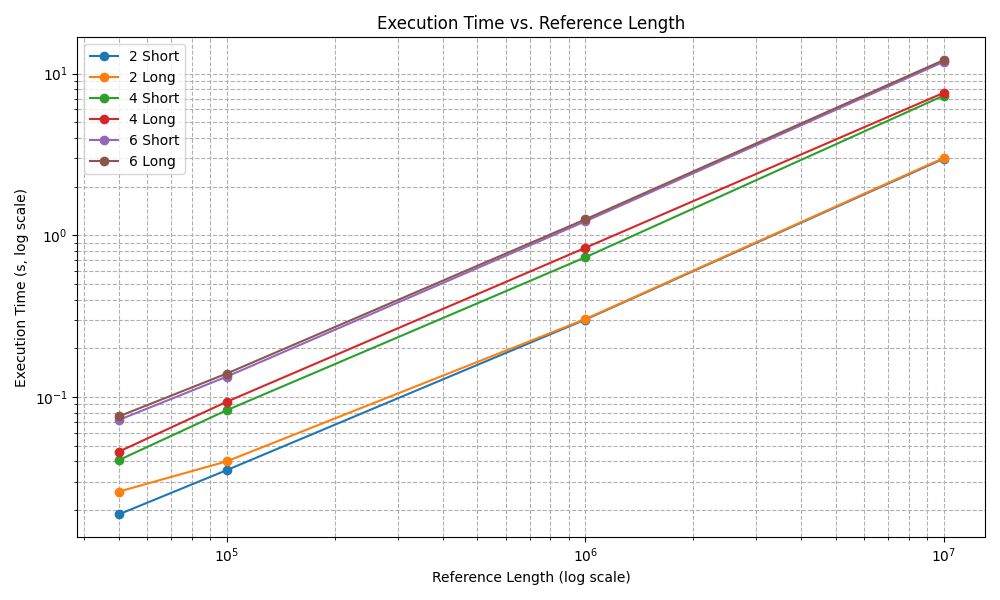
\includegraphics[width=350px]{linearref.png}

  \caption{Execution time as a function of reference length for 2, 4, and 6 inversions, comparing short and long inversions. The plot uses a logarithmic scale on both axes, highlighting the linear relationship between the reference length and execution time, that is consistent with the algorithm's time complexity.}
  \label{fig:refgraph}
\end{figure}

Additionally, the results show that execution times increase almost linearly with the number of inversions \( n \). For instance, at \( r \) = 100000, the time for 2 short inversions was 0.0353 \( s \), while for 6 short inversions, it was 0.1336 \( s \): roughly a 3.7x increase for 3 times the number of inversions.\\
Also evident is a slight but consistent increase in execution time when dealing with longer inversions. For example, at \( r \) = 10000000, the time for 2 short inversions was 0.3009 \( s \), while for 2 long inversions and the same reference length, it was 0.3029 \( s \). The impact of inversion length \( m \) is less pronounced than the impact of \( r \) or \( n \), but still measurable. \\
As \( r \) increases, the difference in execution times between short and long inversions diminishes in relative terms. In fact, at \( r \) = 10000000, the execution time for 2 short inversions is 2.9765 \( s \), while for 2 long inversions is 3.0082 \( s \). The difference is minimal compared to the absolute increase caused by the reference length.

\subsection{With inverted duplications}

Inverted duplications are a type of SV in which a segment of DNA is duplicated and the copy is inserted in the reverse orientation relative to the original. These duplications are often found in genomes and can be associated with various genetic disorders and evolutionary processes \cite{hermetz_large_2014}. In an inverted duplication, the duplicated sequence is typically contiguous with the original, but flipped in orientation, leading to an inverted repeat structure, as summarized in Figure \ref{fig:invd}.

\begin{figure}[h]

  \centering
    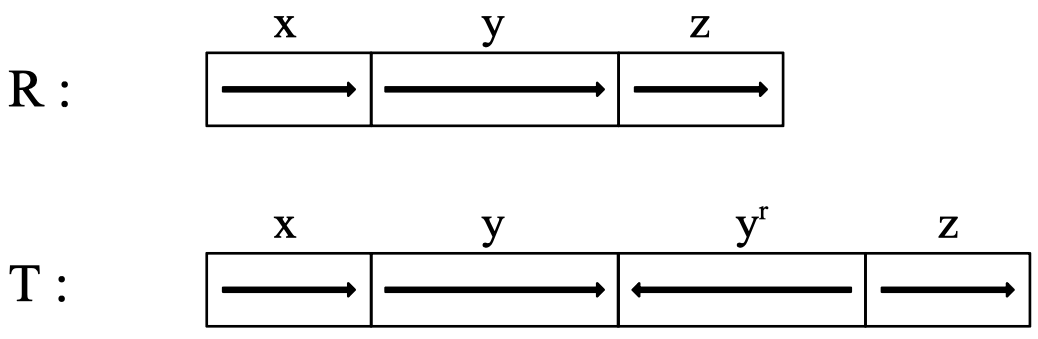
\includegraphics[width=300px]{invd.png}

  \caption{Reference sequence \( R \) and target sequence \( T \) that has undergone an inverted duplication event. In the reference, the sequence consists of three segments, \( x \), \( y \) and \( z \), all oriented in the same direction. However, in the target, the segment \( y \) is duplicated and inserted in the reverse orientation, indicated as \( y^r \).}
  \label{fig:invd}
\end{figure}

In order to generate samples that contain inverted duplications, another \texttt{Python} script was built, \texttt{input\_duplications.py}. It allows setting the reference length, target length, and the start and end indexes of the segment that will be inverted and inserted directly afterward. \\
The experimentation shows that the algorithm can also detect inversions in these situations, since sample-specific strings are detected at the beginning and end of the inverted segment in the target. This segment, when reversed, matches a segment in the reference (see Figure \ref{fig:invd} where, if \( y^r \) is reverted, \( y \) is obtained, which is present in the reference). The next step was to determine the breakpoints, just like in the case without inverted duplications.

\chapter{Conclusions}
\section{Final considerations}
For large reference genomes (e.g., in genomic studies where \textit{r} can be several million base pairs), the algorithm's performance could become a bottleneck unless optimizations specific to handling larger sequences are applied. If many inversions are to be detected (e.g., during large-scale genomic rearrangement studies), the algorithm may need further optimizations in the loop or process that handles inversion detection. 



\section{Future improvements}

\bibliographystyle{unsrt}
\bibliography{bibliography_v2.bib}

\end{document}